\documentclass[a0,portrait]{a0poster}
%\usepackage{alltt}
\usepackage{color}
\usepackage{times}
\usepackage{amsmath,amsfonts,amssymb} % God matematik
\usepackage{a0poster}
\usepackage{pst-node,graphicx} % For graphics, the first is for the background photo. 
\usepackage[utf8]{inputenc} % ÆØÅ pakken
\usepackage[T1]{fontenc} % Font encoding.
%\usepackage[pdftex,bookmarks=true,bookmarksnumbered=true]{hyperref}

%%%%%%%%%%%%%%%%%%%%%%%%%%%%%%%%%%%%%%%%%%%%%%%%%%%%%%%%%%%%%%%%%%%%%%%%%%%%%


\begin{document}
\title{Centralized State Estimation of Distributed Maritime} % Line one of the title
\titletwo{Autonomous Surface Oceanographers} % Line two of the title.
\author{Rasmus L. Christensen, Frederik Juul, Nick \O stergaard, Tudor Muresan, Attila Fodor}
\address{Section for Control and Automation, Department of Electronic Systems, Aalborg University, Denmark$^\dagger$}
\email{\{ralch,nickoe,fjuul,tudor,attila\}@es.aau.dk}

\makeheader
%% Column 1
\begin{center}
\col{
\paragraph{Introduction}
Seaborne measurements are often an expensive and time-consuming task. They could however in many cases have a large impact on the area where they are obtained. At the Fukushima accident in 2011 the area of effect in the water and the safety margin was primarily based on estimates, as only few measurements were available.
The coastal areas around Greenland are another area which could benefit from seaborne measurements as up to date maps are not available. This causes the ships which need to pass near the coast to have a higher safety margin, which in turn lowers the amount of traffic possible. This poster describes parts of the project, and presents results of measurements towards the end \cite{engineer}.

\paragraph{Path Optimization}
The path planning algorithm is based around the train-track transition problem originally solved in \cite{arthur}, which divides the path into straight and turning parts and describes the transition between these using the normalized Fresnel integral, describing an Euler spiral, which allows the ship to maintain a linear acceleration through the turn, thus minimizing the amount of jerk $j$. The two Fresnel integrals are given as in equation (\ref{eq:fresnel}):
\begin{align}
C_F(x) = \int_0^x \cos(t^2)dt,\,\,\,\,S_F(x) = \int_0^x \sin(t^2)dt
\label{eq:fresnel}
\end{align}
The two normalized Fresnel integrals produces the Euler spiral. However, the ship moving along the track can only endure a limited amount of centripetal acceleration $a_\text{centripetal}$, which is a function of the speed of the vessel $v$ and the path curvature $\kappa$. The ship will have a limited angular acceleration $\dot{\kappa}_\text{max} = \alpha_\text{max}$, which results in a scaling $\eta$ of the Euler spiral given by the maximum centripetal acceleration:
\begin{align}
\text{max}\langle a_\text{centripetal}\rangle = \frac{v^2}{r} = v^2 \cdot \kappa \quad , \quad \eta = \frac{\alpha_\text{max}}{v^2_\text{max}}
\end{align}
The threshold $\varepsilon_\text{max}$ can be determined based on a function of the vehicles maximum angular acceleration change $\kappa_\text{max}$ and the maximum centripetal acceleration $a_\text{centripetal}$, thus:
\begin{align}
\varepsilon_\text{max} = \frac{\kappa^2_\text{max}}{2\eta}
\end{align}
If the angle of the turn is lower than the threshold, the turn can be completed in two similar Euler spiral stages. The 3 key points are given by the coordinate sets and are depicted on figure \ref{fig:3points}, where the coordinates are given by equation (\ref{eq:for1}).
\begin{align}
A_3 = (-X_1,Y_1),\, C_3 = (0,\frac{y_d}{\cos(\varepsilon)}),\, E_3 = (X_1,Y_1)
\label{eq:for1}
\end{align}
\begin{figure}
	\begin{center}
		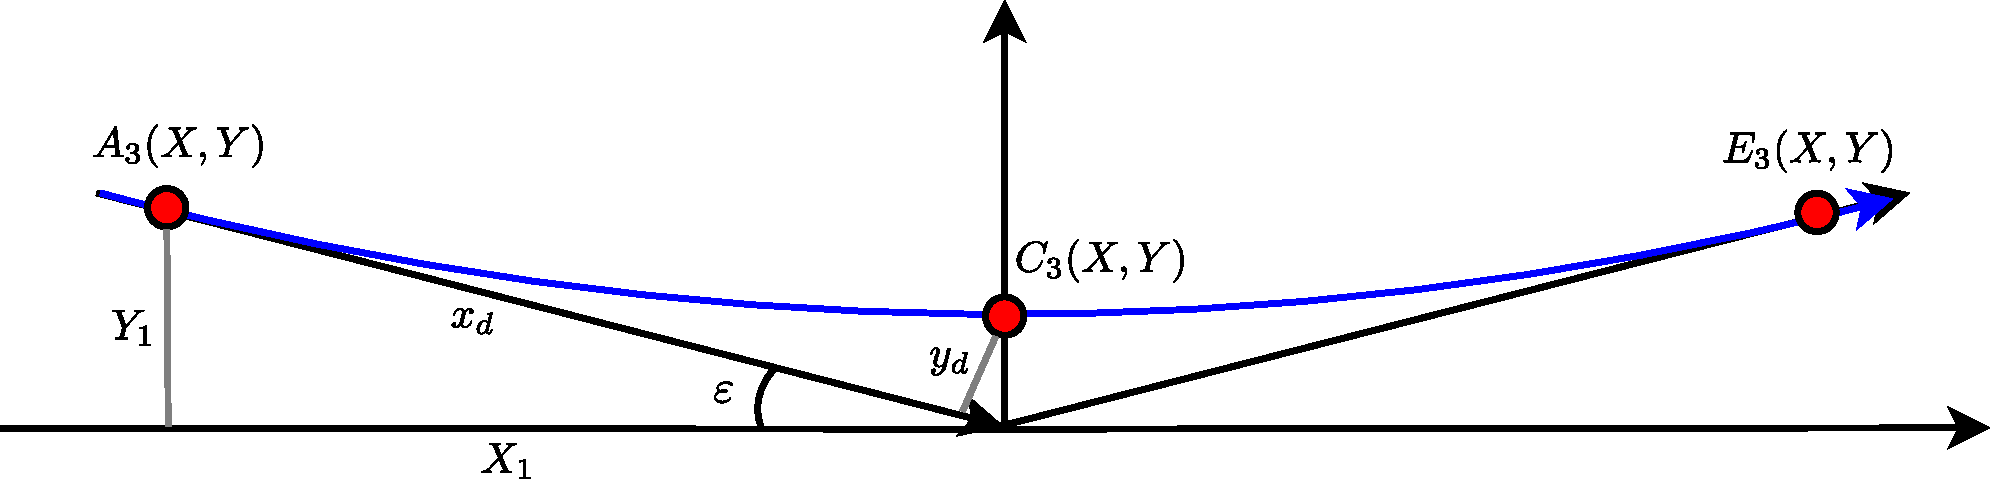
\includegraphics[width=\threecolwidth]{img/3Points} % width of a column is 8.4 cm.
		\caption{Path planning when $\varepsilon$ < $\varepsilon_\text{max}$, the path is composed by two identical but mirrored Euler-spirals. 3 key points are generated, denoted $A_3$, $C_3$ and $E_3$}
		\label{fig:3points}
	\end{center}
\end{figure}
From here, the individual coordinates can be computed by simple trigonometric equations, if the angle of the turn $\varepsilon$ is known. $x_d$ and $y_d$ are the length of the scaled Euler-spiral, when the turn of the spiral equals $\varepsilon$, where $x_d$ and $y_d$ represents the $(x,y)$ coordinate pair of the two normalized Fresnel integral functions with the parameter $t$.
\begin{align}
\varepsilon = \frac{\partial x}{\partial y}f(t) \to [x_d,y_d] = f^{-1}(\varepsilon)
\end{align}
Thus solving for $X_1$ and $Y_1$ gives the following expression as a function of $x_d$ and $y_d$:
\begin{align}
X_1 = x_d \cdot \cos(\varepsilon) + y_d \cdot \sin(\varepsilon),\,\, Y_1 = X_1 \cdot \tan(\varepsilon)
\end{align}

}
%% Column 2
\rput{Center}{
\includegraphics[width=1.9\textwidth]{img/background.pdf}} % Background image
\col{
\paragraph{}
\begin{figure}
	\begin{center}
		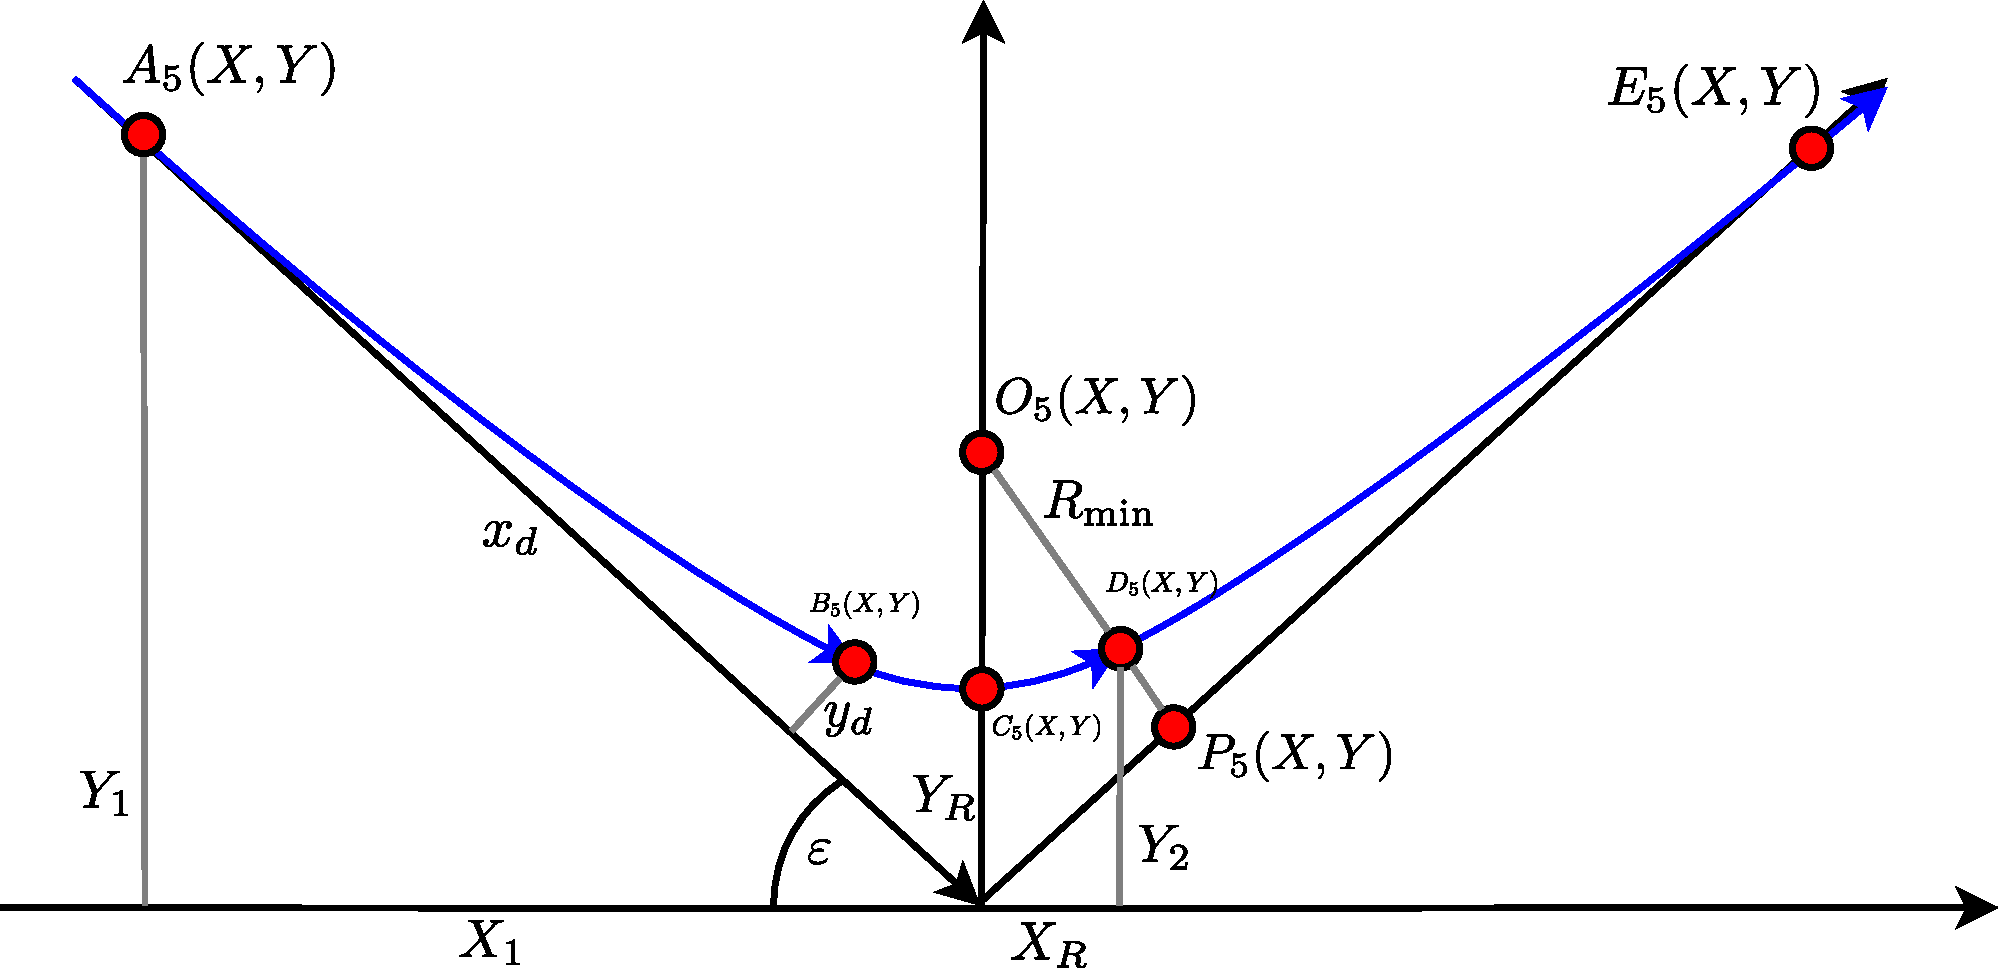
\includegraphics[width=\threecolwidth]{img/5Points}    % The printed column  
		\caption{Path planning when $\varepsilon$ < $\varepsilon_\text{max}$, the path is approximated by a curve and only 3 sub-waypoints are generated, denoted $A_5$, $B_5$, $C_5$, $D_5$ and $E_5$.}  % width of a column is 8.4 cm.
		\label{fig:5points}               
	\end{center}                                 % accordingly.
\end{figure}

If the angle grows larger than $\varepsilon_\text{max}$ the system has to compute five key points, as seen on figure \ref{fig:5points}, due to the ship transitting onto a curve and then back onto the Euler spiral $\text{max}\{\kappa_\text{Euler}\} = \kappa_\text{arc}$. This adds the extra waypoints $B_5$ and $D_5$ which defines the entry and exit points of the curve. The center of the circular path segment is $O_5$ and the radius is $R_\text{min} = \frac{1}{\kappa_\text{max}}$. The coordinates of these waypoints are defined as:
\begin{align}
B_5 = (-X_2,Y_2),\,\, D_5 &= (X_2,Y_2)
\end{align}
Which is still a mirroring of points about the $x=0$ axis, as the entry angle is the same as the exit angle. The number of equations increases, and the individual coordinates for the key waypoints become:
\begin{align}
X_R &= R_\text{min} \cdot \sin(\varepsilon - \varepsilon _\text{max}),\,\, P_X = X_R + y_d \cdot \sin(\varepsilon)\\
X_1 &= P_X + x_d \cdot \cos(\varepsilon),\,\, Y_1 = X_1 \cdot \tan(\varepsilon)\\
P_Y &= Y_1 - x_d \cdot \sin(\varepsilon),\,\, Y_2 = P_Y + y_d \cdot \cos(\varepsilon)\\
O_Y &= R_\text{min} \cdot \cos(\varepsilon - \varepsilon _\text{max}) + Y_2,\,\, R_Y = O_Y - R_\text{min}\\
X_2 &= X_R
\end{align}

\paragraph{State estimation}
To improve the measurements of the ship, a state estimator is implemented, this is based around the two 2 sensors mounted aboard the ship, a GPS and an IMU. The IMU measures the acceleration, the rotational velocity and the magnetic field strength for use in heading calculations. The GPS gives an absolute position reference for use in the control algorithms. The purpose of the estimator, is to give an estimate of $\hat{\vec{x}} = \begin{bmatrix}x & \dot{x} & y & \theta & \omega\end{bmatrix}^T$ where a Kalman filter is used to fuse the IMU and GPS measurements. As a double integration of the IMU results in a large error these measurements are not included in the position estimates directly, but a delayed version is used through the velocity measurements as these also include an absolute version of the velocity from the GPS. This results in the discrete state model for the Kalman filter in equation (\ref{eq:kalmana}):
\begin{align}
\vec{\Phi} = \text{diag}\{\vec{\Phi} _x,\vec{\Phi} _y,\vec{\Phi} _\omega\},\,\, \vec{\Phi}_{x,y,\omega}(k) = \begin{bmatrix}
1 & t_s & 0\\
0 & 1 & t_s\\
0 & \frac{-\beta_{x,y,\omega}}{m,m,I} & 0
\end{bmatrix}
\label{eq:kalmana}
\end{align}
The Kalman filter is implemented as a linear minimum mean square error filter - given by \cite{grewal} where the tuning of the filter, is done using the covariance matrices $\vec{Q}_k$ and $\vec{R}_k$. The input covariance matrix $\vec{R}_k$ has been computed using the following distributions of the force along the $x$- and $y$-axis, and the torque about the $z$-axis. Resulting in the following distributions:
\begin{align}
\vec{F} \sim \mathcal{N}(\vec{\mu_F},\vec{\sigma}^2_F),\,\,\, \tau_z \sim \mathcal{N}(\mu_{\tau},\sigma^2_{\tau})
\end{align}
These parameters for the force is given as follows $\vec{\mu_F} = \begin{bmatrix}5.3544 & 0\end{bmatrix}^T$, $\vec{\sigma}^2_F = \begin{bmatrix}55 & 15\end{bmatrix}$ and the distribution parameters for the torque is $\mu_{\tau} = 0$ and $\sigma^2_{\tau} = 20$. Resulting in the static covariance matrix:
\begin{align}
\vec{R}_k = \text{diag}\{0,0,\sigma^2_{F(1)},0,0,\sigma^2_{F(2)},0,0,\sigma^2_\tau\}
\end{align}
The measurement covariance matrix $\vec{Q}_k$ is a measured estimate of the variances of the sensors.
}
%% Column 3
\col{
\paragraph{}
The distribution of the measurements are considered to be zero mean white noise processes which is defined as $\vec{v}_k \sim \mathcal{N}(\vec{\mu}_v,\vec{\sigma}^2_v)$, giving the covariance matrix as $\vec{Q}_k = \text{diag}\{\vec{\sigma}^2_v\}$. 

\paragraph{Results}
To verify if the computed state estimator works in accordance with the theory, the filter have been tested by walking around the university. Two tests have been performed, one where the system was given all the GPS measurements, the plot on figure \ref{fig:path}a and \ref{fig:error}a) and one where the GPS signal was cut for one minute on figure \ref{fig:path}b and \ref{fig:error}b thus relying only on the IMU measurements.
\begin{figure}
	\centering % Figure input
	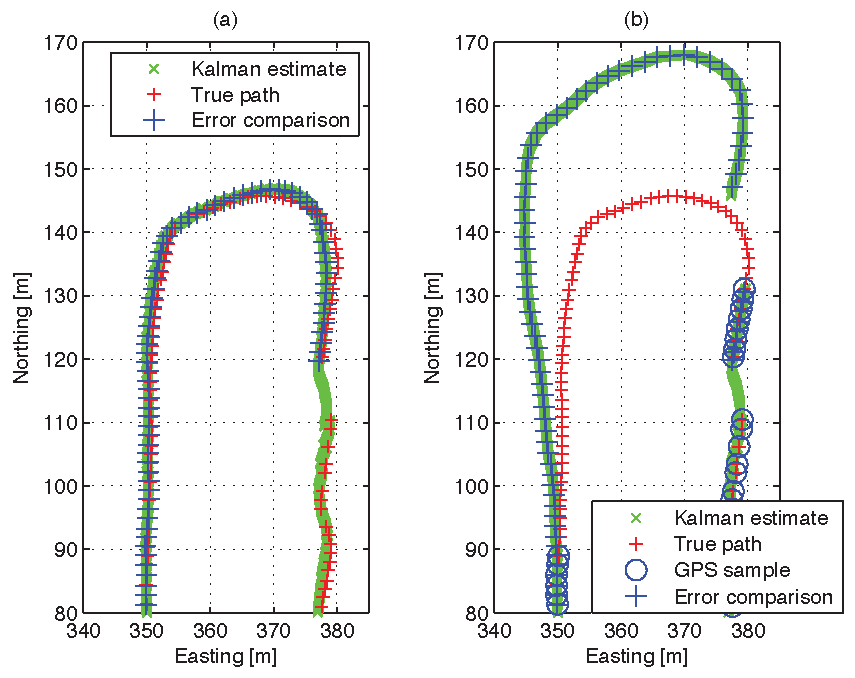
\includegraphics[width=\threecolwidth]{img/track}
  	\caption{(a) is a plot of the system with all GPS samples present. (b) is a plot of the system with a 60 second loss of the GPS signal.}
	\label{fig:path}
\end{figure}
\begin{figure}
	\centering % Figure input
	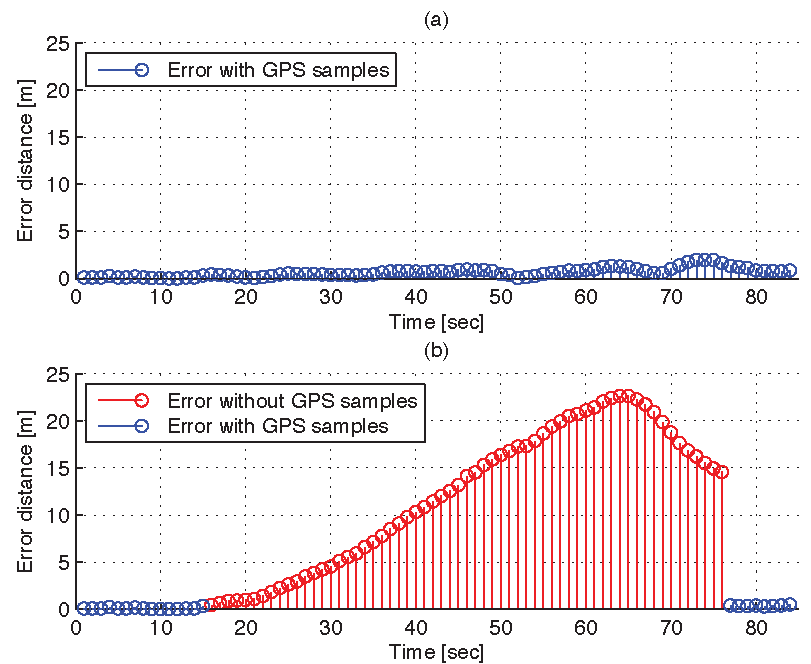
\includegraphics[width=\threecolwidth]{img/error}
  	\caption{(a) is the error plot with all GPS samples present. (b) is a worst case plot of the error with a 60 second loss of GPS signal.}
	\label{fig:error}
\end{figure}


\paragraph{Conclusion}
The figures \ref{fig:path} and \ref{fig:error} illustrates that even though the ship looses GPS measurements for 1 minutes, the ship is still able to follow the path using the IMU data as a reference. The error is expected to be in this range, as the error grows exponentially as it is a double integral of the acceleration and that the accelerometer might not have been completely level, thus increasing the bias of the measurement. And as soon as the GPS comes back online, the estimates converges to the path.

\paragraph{Acknowledgements} A big thanks should be extended to Assistant Professor Carles Navarro Manchón, Aalborg Unviversity, for his help with tuning the Kalman filter. 

\references
\bibliography{litterature}
}
\end{center}

\makefooter
\end{document}





